\chapter{INTRODUÇÃO}

A cada ano, o número de veículos furtados ou roubados no Brasil tem aumentado consideravelmente. Somente em 2016 foram 557 mil veículos furtados no país, contra 510 mil em 2015, o que representa um aumento de 8\% de um ano para o outro, segundo o Fórum Brasileiro de Segurança Pública\footnote[1]{https://goo.gl/n6ajJ2}. Outros números desta instituição apontam que 41\% destes crimes ocorrem nas capitais. A Figura~\ref{fig:roubos} mostra a série histórica de roubos de veículos no Brasil desde 2007, ano em que Fórum Brasileiro de Segurança Pública iniciou a série (os dados referentes a furtos foram contabilizados apenas a partir do ano de 2013) \cite{fbsp2017}.

\begin{figure}[!htb]
\centering
\caption{Veículos Roubados no Brasil por ano.} %legenda
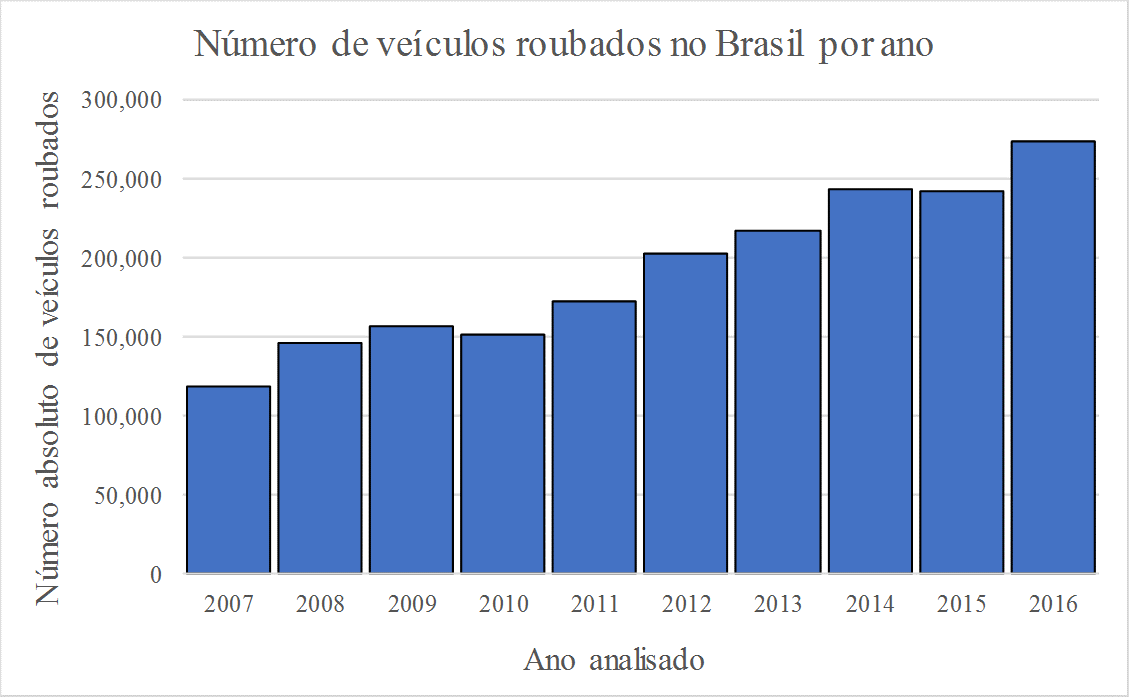
\includegraphics[scale=0.4]{roubosporano.png}\\  % o 0.9 indica 90% do tamanho original
% pdfLaTeX aceita figuras no formato PNG, JPG ou PDF
% figuras vetoriais podem ser exportadas para eps e depois convertidas para pdf usando epstopdf
{\small Fonte: Adaptado de \citeonline{fbsp2017}.} %Fonte da imagem
\label{fig:roubos} %rotulo para refencia
\end{figure}

Estes números contribuem para a discussão de novas formas de prevenção contra roubos e furtos, de interesse de toda a sociedade, em especial proprietários de veículos, seguradoras de bens e autoridades de segurança pública que diretamente sofrem com as consequências deste problema. Tecnologias que evitam este tipo de situação são vistas com bons olhos, principalmente quando funcionam de forma rápida e de tal modo a deter a ação criminosa a tempo de se evitar perdas maiores.

Grande parte dos dispositivos antifurto veicular em pregados atualmente são restritos a sistemas físicos instalados no veículo, tais como travas elétricas e sistemas de alarme, porém sem nenhum sistema de comunicação externo que alerte o proprietário ou as autoridades de segurança. Estes sistemas também são facilmente burlados e consequentemente não impedem o criminoso de cometer o delito.

Em paralelo a este contexto, a indústria automobilística tem experimentado avanços no que diz respeito à conectividade, emprego de sensores de diversas finalidades, que viabilizam a introdução do conceito de \textit{smart vehicles}. Isto significa que os veículos estão cada vez mais \textit{cientes} do ambiente no qual estão inseridos e, consequentemente, podem alertar, aconselhar ou até mesmo intervir em situações ditas de risco aos usuários do mesmo. Hoje existem diversos Sistemas Avançados de Assistência ao Condutor, ou ADAS (\textit{Advanced Driver Assistance Systems}) que auxiliam o condutor na dinâmica de direção, além de otimizarem o consumo energético, entre outras funções que serão abordados posteriormente.

Diante do problema brasileiro de furtos e roubos de veículos e ciente do potencial que os \textit{smart vehicles} têm de solucionar problemas relacionados à dinâmica de direção, este trabalho tem como objetivo propor um sistema de identificação de condutores, ou seja um sistema que saiba discernir entre condutores "autorizados" a conduzir o veículo e um possível criminoso que tenha o tenha furtado ou roubado, tomando as devidas providência para impedir a casualidade. Isto se dará pela identificação de certos padrões de direção, característicos de cada condutor, extraídos de dados provenientes de sensores do veículo e externos a este que modelem a dinâmica de direção e posteriormente submetidos à uma técnica de inteligência computacional que identificará o condutor.

\section{Objetivos}

Este trabalho tem como objetivo investigar técnicas de aquisição e processamento de dados, bem como recursos de inteligência computacional e sua aplicabilidade em um sistema de identificação de condutores, com o intuito de identificar possíveis situações de furto ou roubo. Este sistema fará uso de dados oriundos de sensores presentes no veículo e lidos por meio da interface OBD-II e sensores inerciais embarcados em outros dispositivos. Este sistema resultará no desenvolvimento de um modelo computacional que cumprirá a tarefa de identificação do condutor que opera o veículo. Para tal, foram estabelecidos os seguintes objetivos específicos:

\begin{itemize}
	
	\item Analisar a viabilidade do sistema proposto por meio do uso de banco de dados utilizando o \textit{dataset} do \textit{Hacking and Countermeasure Research Lab} \cite{kwak2016know}, \textit{dataset} UYANIK \cite{Abut2007} e \textit{Driving Behavior Dataset} da PUC-Rio \cite{OLIVEIRAVASCONCELOS2017}.
	
	\item Avaliar técnicas de processamento de dados, de modo a eliminar quaisquer ruídos e erros de leitura, e otimizar a extração de características pela técnica de inteligência computacional, 
	
	\item Após comprovação da viabilidade do sistema, determinar uma técnica de inteligência computacional com aprendizado \textit{online} tendo em vista o melhor desempenho em identificar o condutor. Irá-se avaliar alguns aspectos para a seleção da técnica: 1) a precisão na identificação dos condutores; 2) o custo computacional da mesmo, visto que o sistema poderá potencialmente ser embarcado em uma plataforma limitada computacionalmente; 3) O tempo de processamento até que o condutor seja autenticado, uma vez que quando mais rápido um condutor desautorizado for identificado, maiores a chances de evitar uma ação criminosa.
	
	\item Modelagem e configuração de experimentos com o sistema de aprendizado online, de forma a simular situações reais e testar o desempenho do modelo de identificação.

	
\end{itemize} 

\section{Motivação}

Os avanços dos ADAS em países desenvolvidos têm visado atender as necessidades destes países. Ou seja, países com índices de criminalidade baixa, as fabricantes de automóveis não tem como interesse primário desenvolver sistemas anti-furto, tal qual proposto neste trabalho. É preciso identificar as demandas de cada região e então torna-se mais interessante oferecer funcionalidades que proporcionem ao consumidor maior conforto e segurança.

O Brasil, tradicionalmente, é um importador de tecnologias, sendo assim, consumem-se aqui técnicas que não foram desenvolvidas para atender as necessidades do país, surgindo a demanda pela adaptação de tecnologias ADAS à realidade brasileira. Então, ciente desta lacuna que exite por um sistema anti-furto, aliada ao potencial que ADAS tem a oferecer, um sistema de identificação de condutores traria contribuições enumeradas a seguir:

\begin{itemize}

	\item O sistema de identificação de condutores tem potencial de contribuir na mitigação o problema crônico de roubos e furtos de veículos no Brasil.
	
	\item Os prejuízos anuais causados por roubos e furtos de veículos à população, seguradoras e a mobilização de forças de segurança pública na investigação e repressão à este problema, poderiam ser reduzidos pelo emprego de tal sistema.
	
	\item Do ponto de vista de investigação de acidentes e responsabilização de casualidades, o sistema poderia ser empregado junto com sistemas caixa-preta na investigação de casualidades e responsabilização dos culpados \cite{Barbosa2017}.

\end{itemize}


\section{Estrutura do Trabalho}

Este trabalho está organizado da seguinte forma: O Capítulo~\ref{cap:revisao} apresenta a revisão bibliográfica acerca dos temas que serão abordados ao longo da pesquisa, tais como veículos inteligentes, sistemas avançados de assistência ao condutor (ADAS) e inteligência computacional aplicada à identificação de comportamento de condutores, além da elucidação acerca das ferramentas e técnicas associadas ao desenvolvimento do modelo. No Capítulo~\ref{cap:metodologia}, serão apresentados as etapas de desenvolvimento do sistema proposto, bem como uma breve explanação com base na literatura dos procedimentos que serão adotados. No Capítulo~\ref{cap:resultados} serão indicados quais os resultados esperados ao final do projeto. O Capítulo~\ref{cap:equipe} apresenta a equipe envolvida na pesquisa. O orçamento esperado para o projeto está contido no Capítulo~\ref{cap:orcamento}. Por fim, o Capítulo~\ref{cap:crono} apresenta o cronograma das atividades a serem desenvolvidas.